\documentclass{article}

\usepackage[utf8]{inputenc}
\usepackage[pdftex]{hyperref}
\usepackage{mathtools}
\usepackage{graphicx}
\DeclarePairedDelimiter{\ceil}{\lceil}{\rceil}

\title{Trabalho Prático 0: Operações de Nubby}
\author{Danilo Pimentel de Carvalho Costa\\2016058077}
\date{}

\begin{document}

\maketitle

\section{Introdução}

Este trabalho consiste na implementação do desafio de Bryan de duas formas diferentes: utilizando a matriz de Nubby e a Árvore de Segmentos proposta por Bryan. O objetivo final do trabalho é identificar as possíveis vantagens da abordagem de Bryan para a solução do problema, ou seja, identificar as vantagens de se utilizar a Árvore de Segmentos ao invés da matriz proposta por Nubby.

\section{Solução do Problema}

Tanto a solução proposta por Nubby quanto por Bryan são formas de organizar e pré-calcular os dados a partir das entradas inseridas. Ambos sugerem a criação de uma estrutura de dados que armazene o mínimo, máximo e a soma de todos os intervalos, e que seja atualizada à medida que necessário.

Em ambas as implementações deste projeto foi utilizada uma estrutura para armazenar os dados do intervalo. Ela contém os campos \texttt{min} (valor mínimo), \texttt{max} (valor máximo) e \texttt{sum} (soma dos valores).

\subsection{Matriz de Nubby}

Nubby propôs uma matriz para armazenar os dados de um intervalo. Dado o intervalo $i$, $j$ do vetor de entrada, acessamos a linha $i$ e a coluna $j$ da matriz e encontramos os dados que precisamos na estrutura de dados mencionada.

Após qualquer atualização do vetor de entrada, precisamos recalcular as informações para todos os intervalos. Ou seja, em nossa matriz precisamos passar por todas as linhas e colunas e atualizar as informações de máximo, mínimo e soma de acordo com o vetor de números atualizado.

\subsection{Árvore de Segmentos}

A Árvore de Segmentos proposta por Bryan é uma Árvore Binária Completa\footnote{\url{https://www.hackerrank.com/topics/segment-tree}}, e suas folhas correspondem aos elementos isolados do vetor de entrada (intervalos de tamanho 1). O nó pai de dois nós é a união dos dois intervalos, e suas informações de máximo, mínimo e soma são referentes ao intervalo formado. Assim a árvore é construída até sua raiz, que contém o maior intervalo possível, do tamanho do vetor de entrada.

Dada uma atualização no vetor de entrada implica em uma mudança nos valores de seus elementos, precisamos atualizar os nós folha referentes a estes. Após atualizados, os nós-pai destes são atualizados até raiz da árvore. Deste modo, em uma atualização não precisamos computar novamente toda a árvore, e sim somente os nós afetados pela atualização dos nós-folha.

\section{Análise de Complexidade}

\subsection{Espacial}

O consumo de memória crítico neste problema se refere ao espaço utilizado pela estrutura de dados criada em cada solução.

\subsubsection{Matriz de Nubby}

A complexidade espacial da matriz está ligada à quantidade de linhas e colunas. Seja $n$ o tamanho do vetor de entrada, a matriz criada terá $n$ linhas e $n$ colunas. Logo a complexidade espacial da matriz é $O(n^2)$.

\subsubsection{Árvore de Segmentos}

A complexidade espacial da Árvore de Segmentos está relacionada com a sua quantidade de nós, que por sua vez é calculada a partir do tamanho do vetor de entrada $n$. O cálculo da quantidade de nós é feito da seguinte forma:

\begin{itemize}
\item Se $n$ for uma potência de 2, então a quantidade de nós será $2 \cdot n - 1$.
\item Senão, precisamos encontrar a próxima potência de 2 depois de $n$, que pode ser calculada encontrando o logaritmo de $n$ na base 2, e elevando a 2 o teto do valor encontrado. Assim, a quantidade de nós será $2 \cdot 2^{\ceil[\big]{\log_2 n}} - 1$.
\end{itemize}

Supondo que $n$ não é uma potência de 2, sabemos que o expoente da próxima potência de 2 não passará de ${\log_2 n} + 1$. Assim, a expressão $2 \cdot 2^{\log_2 n + 1} - 1$ pode ser simplificada:
\begin{gather*}
  2 \cdot 2 \cdot 2^{\log_2(n)} - 1 \\
  2 \cdot 2 \cdot n - 1 \\
  4n - 1
\end{gather*}

Deste modo, sabemos que a quantidade de nós da árvore varia de $2n - 1$ a $4n - 1$. Assim, a complexidade espacial da Árvore de Segmentos é $O(n)$.

\subsection{Temporal}
As operações críticas do problema são a criação, a busca e a atualização da estrutura de dados.

\subsubsection{Matriz de Nubby}

A criação da matriz envolve na iteração sobre as linhas e colunas da mesma, além da iteração sobre o intervalo no vetor de entrada. Como visto, a Matriz de Nubby é uma matriz quadrada $n \times n$, e o tamanho máximo do intervalo iterado sobre o vetor de entrada é $n$. Assim, iterando sobre $n$ linhas, $n$ colunas e um máximo de $n$ itens do vetor, a complexidade temporal da criação da matriz é $O(n^3)$.

Uma vez criada, a busca pelos dados de um intervalo de $i$ a $j$ na matriz é feito através dos índices $i$ e $j$, resultando em apenas uma instrução de leitura. Assim, a complexidade temporal da busca na matriz é $O(1)$.

A atualização dos dados da matriz consiste na reconstrução da mesma com os dados do vetor de entrada atualizados. Assim, a partir do raciocínio utilizado na criação da matriz, podemos também concluir que a complexidade temporal da atualização da matriz é $O(n^3)$.

\subsubsection{Árvore de Segmentos}

A criação da árvore envolve a criação de todos os nós e a computação dos valores armazenados nestes, e sua complexidade está relacionada à quantidade de nós. Como vimos na análise espacial, a quantidade de nós da árvore varia de $2n - 1$ a $4n - 1$. Assim, a complexidade temporal da criação da árvore é $O(n)$.

A busca pelos dados de um intervalo na árvore feita através da sobreposição do intervalo do nó e do intervalo especificado:

\begin{itemize}
\item Começando pela raiz, se a sobreposição for total, encontramos o nó correspondente ao intervalo buscado. No caso da matriz, o intervalo é o maior possível, e as informações já se encontram na raiz. Este é o melhor caso, e a complexidade temporal é $O(1)$, por que só precisamos recuperar os dados da raiz;
\item Se a sobreposição for parcial, a busca se estende para os 2 nós-filhos do nó em questão;
\item Se não houver interseção alguma entre os intervalos do nó e da busca, a busca não se estende para os filhos deste nó.
\end{itemize}

O pior caso acontece quando a busca se estende até os nós-folha. Neste caso, o algoritmo percorre um caminho correspondente à altura total da árvore. A altura $h$ da árvore é dada por $h = \log N$\footnote{\url{http://www.dgp.toronto.edu/people/JamesStewart/378notes/09treeHeight/}}, sendo $N$ o número de nós da árvore. Como visto, a complexidade do número de nós da árvore é $O(n)$, sendo $n$ o tamanho do vetor de entrada, concluímos que a complexidade temporal no pior caso é $O(\log n)$.

A atualização da árvore consiste na mudança dos valores dos nós-folha correspondentes ao itens que estão contidos no intervalo a ser atualizado. Assim, para chegar ao nó-folha, precisamos percorrer um caminho do tamanho da altura da árvore. Assim, a partir do raciocínio do pior caso da busca, também podemos concluir que a complexidade temporal da atualização é $O(\log n)$.

\section{Análise Experimental}

Podemos fazer alguns experimentos para determinar se a Análise de Complexidade realmente se confirma quando os programas são executados. Para analisar o comportamento e a variação do tempo de execução dos programas, foi utilizada a seguinte estratégia: foram gerados arquivos de entrada com entradas aleatórias e tamanho crescente do vetor. Para cada entrada gerada, eram feitas as seguintes variações: um arquivo sem nenhuma operação, um arquivo com operações de atualização e um arquivo com operações de busca.

As variações nos tipos de arquivos de entradas foram feitas para analisar como as operações influenciam no tempo de execução. Assim, podemos confirmar as complexidades das operações e do tempo de criação das estruturas de dados.

Com as entradas aleatórias geradas, é possível ver como o tempo de execução varia, coletar estes dados e plotar gráficos que nos ajude a analisar o crescimento do tempo. As seguintes subseções mostram os resultados das análises.

\subsection{Matriz de Nubby}

A dificuldade encontrada na análise experimental da matriz foi o alto custo computacional que a criação da estrutura demanda. É visível na execução dos programas que a Matriz de Nubby tem um gargalo grande quando o tamanho da entrada aumenta.

Assim, pra superar esta dificuldade, foram geradas entradas aleatórias com tamanho do vetor de entrada de até 500 posições. Tal número foi escolhido arbitrariamente depois de algumas análises. O seguinte gráfico foi obtido a partir dos tempos de execução:

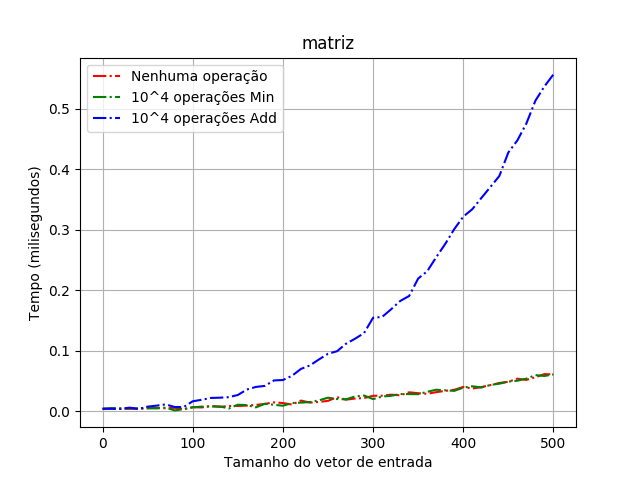
\includegraphics[scale=0.70]{matriz}

Podemos ver como o problema com a solução de Nubby é realmente a computação de toda a matriz após uma atualização do vetor de entrada. O alto custo para se computar a matriz causa um gargalo que cresce exponencialmente de acordo com a entrada, como se pode observar no gráfico obtido.

A grande vantagem da utilização da matriz é a busca por informações de um intervalo. Confirmamos a teoria de que a complexidade temporal das operações de busca na matriz é $O(1)$ observando que mesmo com tantas operações, o tempo de execução do programa quase não é alterado e se aproxima do tempo necessário para a criação.

\subsection{Árvore de Segmentos}

A dificuldade de se analisar experimentamente a Árvore de Segmentos está no fato de que a quantidade de operações que se gasta para se criar a estrutura varia muito de acordo com o tamanho do vetor de entrada. O tamanho do vetor utilizado para se armazenar a árvore pode variar de $2n - 1$ a no máximo $4n - 1$, dependendo de $n$. A fim de obter uma continuidade na criação da árvore, os tamanhos dos vetores de entrada dos arquivos são sempre potências de 2.

Para se obter uma distanciação dos tempos de execução sem nenhuma operação para com operação, a quantidade de operações foi fixada arbitrariamente em $10^5$.

O resultado obtido com esta escolha de parâmetros para o programa está representado no gráfico a seguir:

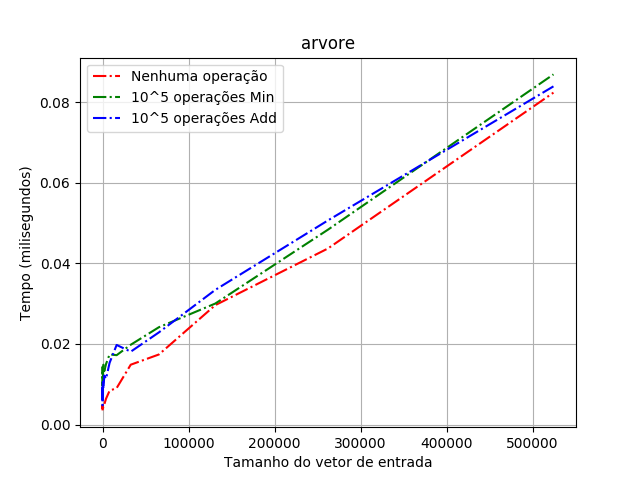
\includegraphics[scale=0.70]{arvore}

A partir da análise dos resultados mostrados no gráfico, podemos perceber que a complexidade temporal $O(n)$ de criação da Árvore de Segmentos se confirma. A curva traçada em vermelho se aproxima de uma reta e cresce linearmente de acordo com o tamanho da entrada.

As curvas correspondentes a operações de busca e atualização também confirmam a teoria da complexidade temporal $O(\log n)$. Note o crescimento rápido para entradas menores e estabilização após o teste com entradas maiores, fazendo com que se aproxime bem de uma curva correspondente à função $O(\log n)$.

\section{Conclusão}

A partir da Análise de Complexidade e da Análise Experimental podemos ver que mesmo que a busca na Matriz de Nubby seja mais rápida em relação à Árvore de Segmentos, todo o processo de criação e atualização da matriz é muito custoso, sendo a mais provável causa do gargalo visto com casos de teste em que o tamanho da entrada é grande. Assim concluímos que a implementação do problema utilizando a Árvore de Segmentos é a melhor opção.

\end{document}
